\chapter{Background}
\label{chap:technical}

\section{The Lambda Calculus}
\newcommand{\lcalc}{$\lambda$-calculus}
\newcommand{\lCalc}{$\lambda$-Calculus}
\newcommand{\fto}{\rightarrow}
The lambda calculus (\lcalc) was described by Alonzo Church in 1936~\cite{church1936unsolvable}. 
\sam{too terse: what is the lamda calc? (model of computation). Why is it important / interesting to this project?}
Below is a definition of the \lcalc~\cite{barendregt2013lambda}.

\sam{you can't jump straight into this} 
\begin{definition}[The \lcalc]
    The set of $\lambda$-terms, notation $\Lambda$, is built up from an infinite set of variables $V={v,v',v'',...}$ \sam{here you say v, but below you use x} using application and (function) abstraction: \sam{functions? application? abstraction? what are these? I recommend getting Sarah to have a look a this BG to see what a non-PL person needs to know}
    \begin{alignat*}{3}
    &x \in V                 \quad && \implies \quad && x \in \Lambda\\
    &M,N \in \Lambda         \quad && \implies \quad && (M N) \in \Lambda\\
    &M \in \Lambda, x\in V   \quad && \implies \quad && (\lambda x. M) \in \Lambda 
    \end{alignat*}
    Using abstract syntax one may write the following:
    
    \begin{alignat*}{3}
    &V       && ::= \; && v \mid V'\\
    &\Lambda && ::= \; && V \mid (\Lambda\Lambda) \mid (\lambda V\Lambda)
    \end{alignat*}
    \sam{I dont think the way you have done variables is standard, i know you dont wanna plagurise, but this is such a basic thing that its better to cite where you got the AST from than tweek to get your own}
\end{definition}

We shall also use the following conventions:

\begin{definition}[The \lCalc\ Conventions]$\ $\vspace{-0.5cm}
    \begin{enumerate}
        \item \(x, y, z,...\) denote arbitrary variables.
        \item We may omit outermost parenthesis.
        \item Nested abstractions can be grouped. For instance, if we were to write the term $\lambda x \;y. M$, we would mean $(\lambda x . (\lambda\;y. M))$.
        \item We assume that the body of an abstraction extends as far to the right as possible. For instance, the term $\lambda x. M\;N$ means $(\lambda x. (M\;N))$ and not $((\lambda x. M)\;N)$. \sam{is this case you have used the standard thing, but I'd cite where you got these conventions from}
    \end{enumerate}
\end{definition}

\newcommand{\BetaReduce}{\rightarrow_\beta}
\subsection{Reduction}
The \lcalc\ is evaluated by $\beta$-reduction. This is where an abstraction is applied to a value. The result of applying an abstraction to a term is the body of the abstraction, with the all free \sam{what do you mean by free?} instances of the abstracted variable are substituted with the term the abstraction was applied to. Below is the definition of how this substitution works, followed by the definition of $\beta$-reduction. 

\begin{definition}[Substitution of free variables in terms of the \lcalc]$\ $\vspace{-0.5cm}
\begin{alignat*}{3}
&x[x::=N]                           \quad && \equiv \quad && N\\
&y[x::=N] \text{ where } y \ne x    \quad && \equiv \quad && y\\
&(M_1 M_2)[x::=N]                   \quad && \equiv \quad && (M_1[x::=N]) (M_2[x::=N])\\
&(\lambda y.M)[x::=N]                \quad && \equiv \quad && \lambda y.(M[x::=N])
\end{alignat*}  
\end{definition}

\begin{definition}[$\beta$-Reduction of the \lcalc]$\ $\vspace{-0.5cm}
\begin{alignat*}{3}
&x                 \quad && \BetaReduce \quad &&        x\\
&\lambda x.M       \quad && \BetaReduce \quad &&        \lambda x.M\\
&(\lambda x.M) N   \quad && \BetaReduce \quad &&        M[x::=N]
\end{alignat*}    
\end{definition}

\begin{definition}[Normal Form]
A term is said to be in normal form if it cannot be $\beta$-reduced
\end{definition}

\sam{these are all standard, so you should cite where they come from and explain them. Spend more time on reduction, because that will be key later}
\sam{this section is very dry. why do we want to learn about lambda calc? well we are writing an evaluator, so to understand what that means we need to understand syntax and evaluation, so lets looks at the lambda calc as a small example. It makes the intro of lambda calc more active and motivated, rather than a bunch of dry definitions, instead its a small example of what we will do later, that is background cos its pre-defined and not implemented we are just exploring the ideas we will implement}

\subsection{Types}
\sam{para generally motivating types}

The \lcalc\ that we have discussed so far is untyped. This means that any $\lambda$ term can be applied to any other term. When a term can no longer be $\beta$-reduced (i.e. no further reductions are possible), we say it is a value. This is why $\beta$-reduction is often referred to as \textit{evaluation} — it is the process by which terms are reduced to their final, fully evaluated form (i.e. values).

\sam{i havent read further of lambda calc, cos i think my above advise applies here too. 1. you are burdened with too much knowledge so you keep jumping into the middle of an explanation 2. it is unclear why we are learning about types 3. remember lambda calc is a whole 3rd year course, and you've seen how long stevens notes are, we cannot replicate that so we need to highlight to the user what is important to understand about the lambda calc for just this project}

If we were to extend our \lcalc\ with a new sort of term, an integer literal (something commonly done, especially when building up to discussing practical functional languages) \[\dots, -2, -1, 0, 1, 2, \dots\] we could say that these values are members of a set of values $Int$. It would be useful for us to be able to assert that a term eventually evaluates to one of these $Int$s. The \lcalc\ terms that evaluate to a value in the set of $Int$s can all be said to have `type' $Int$. More generally: 

\begin{quote}
`Saying that `a term $t$ has type $T$' (or `$t$ belongs to $T$,' or `$t$ is an element of $T$') means that $t$ `obviously' evaluates to a value of the appropriate form - where by `obviously' we mean that we can see this statically, without doing any evaluation of $t$' \cite{pierce2002types}
\end{quote}

\subsubsection{Functions}
We want to be able to express the types of functions. The term \(\lambda x. x\) can be said to have type \(T \fto T\), as it takes in a term of type $T$ and returns the same term, which still has type $T$.

A more complex term \(\lambda x\;y.x\) can be said to have type \(T \fto (U \fto T)\); If we give it a term $M$ of type $T$, it would return the function \(\lambda y.M\) which takes whatever is given to it (represented by $U$) and returns $M$ which has type $T$. 

By convention, $\fto$ is right associative so way may omit the right most parenthesis. 

\subsubsection{Typechecking: Well typed programs do not go wrong}
In this extended value of the lambda calculus, the set of valid values $V$ is:
\[
V ::= \lambda x. M \mid \dots \mid -2\mid -1\mid 0\mid 1\mid 2\mid \dots 
\]

The evaluation of an \lcalc\ expression is said to have `gone wrong' if it gets to a normal form that is not a valid value.

Let us consider the expression and its reduction
\[
(\lambda x. x\;x) \;1 \BetaReduce 1\;1
\]
\noindent The reduction is not a valid value.

We will now attempt to derive the type of the parameter $x$, in order to show that it is untypeable.
As $x$ here is applied to itself, it must be some kind of function that takes a term $x$ of with type $T$ and then applies it to itself. This means that $T = T \fto U$ which is absurd. This means that this is `untypeable'. Indeed, it is clearly never possible to type an expression where a term is applied to itself. If this was a real programming language, when it got to the normal form \(1\;1\), it would be some form of runtime error. We can see that only allowing typeable terms would have prevented us from creating a term that does not evaluate in this case. 

In general, \textbf{well typed programs do not go wrong} \cite{MILNER1978348}. Therefore, if we are able to exclude all terms in our functional language that are untypeable, we will be able to guarantee that it does not go wrong, and thus prevent these runtime errors. 

The system that looks at a program to decide whether it is well typed is called the \textbf{typechecker}. Types can often also be inferred without specific assignments, which is called \textbf{type inference}.

\section{Haskell: A Functional Programming Language}
\sam{why are we talking about Haskell? we need to talk about SFL!}
Functional programming languages are programming languages where `computation is carried out entirely through the evaluation of expressions' \cite{hudak1989conceptionfunctionalprogranning}. Functional programming languages are based on the lambda calculus. In this section, we will only discuss one example: Haskell. 

Haskell is a very prominent functional programming language that is widely taught. It is a programming language specifically designed to be suitable for teaching \cite{hudak2007history}. This dissertation involves the development of a programming language with some similar features to Haskell, so the corresponding Haskell features and ideas will be introduced here. 

\subsection{Declarations}
Haskell, along with most other languages, provides the facility to name functions and values for reference elsewhere in the program. These can be typed, but the types can almost always be inferred. 

Some examples of these declarations, all typed for clarity, are below. For instance, the top level declaration
\begin{verbatim}
x :: Int
x = 5
\end{verbatim}
means that $x$ is equal to $5$. We can also name lambda functions:
\begin{verbatim}
add :: Int -> Int -> Int
add = \x y -> x + y
\end{verbatim}
This can be shortened to:
\begin{verbatim}
add :: Int -> Int -> Int
add x y = x + y
\end{verbatim}

\subsection{Polymorphic functions}
In Haskell, functions can be written that operate on values of various types. A simple argument is 

\begin{verbatim}
id :: a -> a
id x = x
\end{verbatim}
\noindent which simply returns its argument. `a' in the type signature represents any type, and can be substituted for any type. The two `a's must be the same however, mandating that the argument and the return value must be the same type.  

\subsection{User Defined Algebraic Data Types}
\label{bg:haskell_udt}
Many languages, including Haskell, have Algebraic Data Types allowing us to `Compose' other data types. The set of all values of an algebraic data type is isomorphic to an expression involving the sets of values of their constituent types combined using `set algebra' operations. Haskell allows for `union' and `product' types.  

Haskell allows users to define their own algebraic data types using the \lstinline[language=SFL]|data| keyword. For instance, booleans can be defined as 

\begin{lstlisting}[language=SFL_unboxed_noprelude_notypes]
data Bool = True | False
\end{lstlisting} 

\noindent This data definition creates a type $Bool$ with two data constructors, \verb|True| and \verb|False|. These data constructors are zero-ary. We can also have data constructors that have arguments. 

An example of a union type in Haskell is the tagged union \begin{lstlisting}[language=SFL_unboxed]
data Shape = Circle Int | Rectangle Int Int
\end{lstlisting} 
\noindent which is isomorphic to the type \(Int \cup (Int \times Int)\). 

An example of a product type is the tuple \((Int, Bool)\): the set of all possible values of this type is isomorphic to the Cartesian product of the set of all values of \(Int\) and the set of all values of $Bool$. Most languages have product types, which often take the form of structs or tuples. 

\subsection{Polymorphic Types and Kinds}
Haskell includes polymorphic types. These are `types that are universally quantified in some way over all types' \cite{hudak1992gentle}. 

One example is the type constructor $Maybe$, written as \(Maybe\;a\). This is first-order polymorphism, as opposed to higher-order polymorphism where a type can be an `abstraction over type constructors'. \cite{yallop2014lightweightpoly}. Here, \(Maybe\) is not a type in itself, but it represents a constructor that takes a type, and returns a concrete type. 

The `Type of a Type' is its \emph{kind} \cite{pierce2002types}. For example, the type constructor $Maybe$ has the kind $* \fto *$. This notation looks similar to how functions over values are defined, indicating that it behaves like a function, but at the type level rather than the value level. If we were to apply the constructor \(Maybe\) to the concrete type \(Int\), the resulting type would be the concrete type \(Maybe \;Int\). 

`Either' is a type constructor with the kind $* \fto * \fto *$, meaning it takes two concrete types and returns a concrete type. 

\subsection{Pattern Matching}
\label{bg:haskell_pattern_match}
Haskell allows us to do pattern matching, allowing conditional execution based on whether a term matches a given form. The following function would have different results depending on whether the input value was 0 or another number

\begin{verbatim}
isZero :: Int -> Bool
isZero 0 = true
isZero _ = false
\end{verbatim}

\noindent The underscore `\verb|_|' represents a wildcard pattern that matches anything. In this case, it matches any $Int$ that is not $0$. We can match more complicated expressions, and assign variables throughout the pattern.

\todo{ADD SYNTAX HIGHLIGHTING}
\begin{verbatim}
data SomeValues a = One a | Two a a | Three a a a | Four a a a a

valuesToList :: SomeValues a -> [a]
valuesToList (One x) = [x]
valuesToList (Two x1 x2) = [x1, x2]
valuesToList (Three x1 x2 x3) = [x1, x2, x3]
valuesToList (Four x1 x2 x3 x4) = [x1, x2, x3, x4]
\end{verbatim}

\noindent In the first match case of \verb|valuesToList|, we assign the variable $x$ when matching the pattern. In the second, we assign \verb|x1| and \verb|x2| etc. 

\section{Rust}
\label{bg:rust}

This project is written in rust. \sam{why? motivate} Some of the decisions made, particularly in the implementation of the AST, require an understanding of Rust, especially the memory management model.

`Ownership' is an important concept. The rules of ownership \cite{rust_book}:
\begin{itemize}
    \item Each value in Rust has an owner.
    \item There can only be one owner at a time.
    \item When the owner goes out of scope, the value will be dropped.
\end{itemize}   

If a value is owned in one scope, but another scope needs to read/write it, we may use a reference to the value. The rules of references \cite{rust_book}:
\begin{itemize}
    \item At any given time, you can have either one mutable reference or any number of immutable references. 
    \item References must always be valid.
\end{itemize}

These rules ensure that immutable references are to things that don't change, and all references are always to things that exist.

\section{Frontend Technologies}
\label{bg:frontend}
\label{bg:pwa}
\begin{itemize}
    \item Vite
    \item React
    \item NPM
    \item PWAs
\end{itemize}


\section{Web Assembly} \label{bg:wasm}
This project runs entirely within the browser, despite being written in Rust. This is due to the fact that it compiles to web assembly. Automated tools exist for the generation of JavaScript bindings around Rust functions/types, but this process places certain restrictions around their arguments and return type, or attributes. We will discuss this here to allow us to refer to these restrictions, and also to explain the process of compiling and using Rust code in a modern web browser. 

Web Assembly 2.0 is a 32 bit target \cite{WebAssemblyCoreSpecification2}. This means we only have 4 GB of addressable memory. The Rust compiler is based on LLVM, which provides a web-assembly compilation target. The Rust compiler has a toolchain around this compilation target [REFHERE: rust WASM toolchain], that allows for easy compilation to web-assembly. However, this only creates a binary blob, which requires more work to make interoperable with our JavaScript build system (Vite). We must do two things to achieve interoperability:
\begin{itemize}
    \item Incorporate it into our build so it can be served with it.
    \item Load the WASM package in a way that allows for us to call the functions.
\end{itemize}
Producing an NPM package with some JavaScript functions that call the WebAssembly functions would achieve both of these goals. However, if we wish to use TypeScript, we must create a separate type definition file that contains the types of all of the JavaScript wrapper functions around the WASM functions. This would be difficult to maintain manually as we would have to update it every time we made a change to the public interface of our rust library. 

Fortunately, the rust crate \verb|wasm-bindgen| provides macros that generate a whole NPM package, including TS bindings, automatically. This package can then be added as a dependency to an NPM app that provides a website, and the functions within it can [TODO: WASM-bindgen vs WASM pack?]

\paragraph{wasm-pack}
\label{bg:wasm-pack}

\section{Existing systems}
Below are the most relevant existing systems 
% https://dl.acm.org/doi/pdf/10.1145/1480828.1480845
% lit review  in previous diss: https://research.ou.nl/ws/portalfiles/portal/31271878/Nicasi_K_IM9906_AF_SE_scriptie_PURE.pdf
% \subsection{WinHIPE}
% https://dl.acm.org/doi/pdf/10.1145/1273039.1273042

\subsection{Duet, and Duet Delta}

\subsection{$\lambda$-Lessons}
\newcommand{\llessons}{$\lambda$-Lessons}

\llessons\ is:

\begin{quotation}
`A short, interactive lesson that teaches core functional programming concepts. It was designed to transform the way you think about performing operations on lists of things, by showing you how functions are executed' \cite{lambdalessons}
\end{quotation}

\noindent\llessons\ is a very effective demonstration of `map', `foldr' and `foldl'. It is unfortunate I only found out about it at the end of phase 4 of the project, otherwise this project would have potentially gone in a different direction in terms of UI. Despite the fact that my project did not take inspiration from this system, it would be remiss not to mention it. 

\begin{figure}[h]
    \centering
    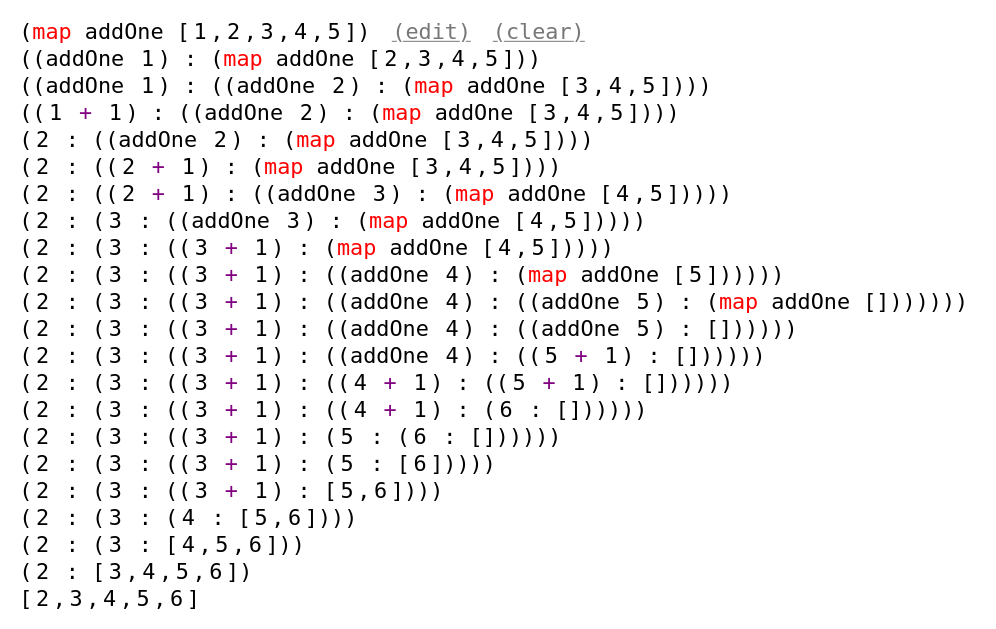
\includegraphics[width=\linewidth]{images/LLessonsMap.png}
    \caption{Evaluation of `\sflinline{map addOne [1, 2, 3, 4, 5]}' with \llessons}
\end{figure}

However, my SFL Explorer is very different to \llessons. 

% https://stevekrouse.github.io/hs.js/